\documentclass{article}

% For math environments
\usepackage{amsmath, amsfonts}
% For links
\usepackage[colorlinks=true,
    linkcolor = blue,
    urlcolor  = blue,
    citecolor = blue,
    anchorcolor = blue]{hyperref}
% Put space between paragraphs
\usepackage{parskip}
% For figures
\usepackage{tikz}
% Set the margins to not be ridiculous
\usepackage[margin=0.75in]{geometry}
% For multiple columns
\usepackage{multicol}
% For controlling enum/itemize spacing and indentation
\usepackage{enumitem}
% More math symbols
\usepackage{amssymb}
% To change enumerate labels

% For tikz plots
\usepackage{pgfplots}
% This isn't needed but avoids a compiler warning
\pgfplotsset{compat=1.16}

% Allow multi-line equations to be broken across pages
\allowdisplaybreaks

% Use @ as a letter
\makeatletter

% Scale down all tikz coordinates while maintaining font size
\tikzset{every picture/.style={scale=0.45, every picture/.style={}}}


% Macros
% Monospace code
\def\code#1{\texttt{#1}}

% Greek letters
\def\a{\alpha}
\def\b{\beta}
\def\g{\gamma}
\def\d{\delta}
\def\D{\Delta}

% Commands that make life easier
\newcommand\gath[1]{\begin{gather} #1 \end{gather}}
\newcommand\ali[1]{\begin{align} #1 \end{align}}
\newcommand\parens[1]{\left( #1 \right)}
\newcommand\squares[1]{\left[ #1 \right]}
\newcommand\braces[1]{\left\{ #1 \right\}}
\newcommand\angles[1]{\left\langle #1 \right\rangle}
\newcommand\deriv[2]{\frac{d #1}{d #2}}
\newcommand\abs[1]{\left| #1 \right|}
\newcommand\floor[1]{\left\lfloor #1 \right\rfloor}
\DeclareMathOperator{\lcm}{lcm}
\def\non{\nonumber \\}

% Multiline equation space
\def\mlesp{\hspace{1.2cm}}

% For grid diagrams
\newcommand\gridbox[3]{\draw (#1,#2) rectangle (#1+1,#2+1) node[pos=.5] {#3};}
\newcommand\gridboxh[3]{\draw[fill=red!20] (#1,#2) rectangle (#1+1,#2+1) node[pos=.5] {#3};}
\newcommand\gridboxb[3]{\draw[fill=black] (#1,#2) rectangle (#1+1,#2+1) node[pos=.5] {#3};}
\newcommand\gridsym[3]{\node at (#1+0.5,#2+0.5) {$#3$};}
\newcommand\gridblank[2]{\filldraw[draw=gray, color=gray] (#1,#2) rectangle (#1+1,#2+1);}
\newcommand\gridcirc[2]{\draw (#1 + 0.5,#2 + 0.5) circle (0.25);}
\newcommand\cwlab[3]{
  \def\dd{0.15}
  \draw (#1 + \dd - 0.03, #2 + 1 - \dd) node {\scriptsize #3};
}

\def\bbw{3.5}
\def\bbh{2}
\newcommand\bigbox[3]{\draw (#1*\bbw,#2*\bbh) rectangle (#1*\bbw+\bbw,#2*\bbh+\bbh) node[pos=.5] {#3};}
\newcommand\bbtextr[3]{\node[right] at (#1*\bbw,#2*\bbh+0.5*\bbh) {#3};}
\newcommand\bbtextb[3]{\node[align=center] at (#1*\bbw+0.5*\bbw,#2*\bbh+0.5*\bbh) {#3};}

% Box puzzle stock answer
\newcommand\boxans[1]{
  Logic was used to deduce the solution:

  #1

  This was verified using Python as well as shown to be unique with a brute force approach.
}

% Multiple numbers
\newcommand\mn[1]{$#1$'s}

% Commands for problems
\newcommand\problem[4]{
  \section*{#1}

  Question: #3
  
  Answer: #2
  
  Explanation: #4
}
\newcommand\aproblem[4]{\problem{Dec #1}{#2}{#3}{#4}}
\newcommand\cproblem[4]{\problem{Problem #1}{#2}{#3}{#4}}

\def\advent@xxiv@i{
  Eve writes down five different positive integers.
  The sum of her integers is $16$. What is the product of her integers?
}

\def\advent@xxiv@ii{
  $14$ is the smallest even number that cannot be obtained by rolling two $6$-sided dice and finding the product of the numbers rolled.

  What is the smallest even number that cannot be obtained by rolling one hundred $100$-sided dice and finding the product of the numbers rolled?
}

\def\advent@xxiv@iii{
  There are $5$ ways to write $5$ as the sum of positive odd numbers:
  \begin{itemize}
    \item $1 + 1 + 1 + 1 + 1$
    \item $1 + 1 + 3$
    \item $3 + 1 + 1$
    \item $1 + 3 + 1$
    \item $5$
  \end{itemize}

  How many ways are there to write $14$ as the sum of positive odd numbers?
}

\def\advent@xxiv@iv{
  The geometric mean of a set of $n$ numbers is computed by mulitplying all the numbers together, then taking the $n$th root.
  The factors of $9$ are $1$, $3$, and $9$.
  The geometric mean of these factors is
  \gath{
    \sqrt[3]{1 \times 3 \times 9} = \sqrt[3]{27} = 3
  }
  What is the smallest number where the geometric mean of its factors is $13$?
}

\def\advent@xxiv@v{
  The sum of $11$ consecutive integers is $2024$.
  What is the smallest of the $11$ integers?
}

\def\advent@xxiv@vi{Put the digits 1 to 9 (using each digit exactly once) in the boxes so that the sums are correct. The sums should be read left to right and top to bottom ignoring the usual order of operations. For example, 4+3×2 is 14, not 10. Today's number is the product of the numbers in the red boxes.
  The number $n$ has $55$ digits.
  All of its digits are $9$.
  What is the sum of the digits of $n^3$?
}

\def\advent@xxiv@vii{
  What is the obtuse angle in degrees between the minute and hour hands of a clock at 08:22?
}

\def\advent@xxiv@viii{
  It is possible to arrange $4$ points on a plane and draw non-intersecting lines between them to form $3$ non-overlapping triangles:

  \begin{center}
    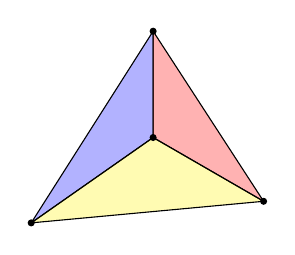
\begin{tikzpicture}
      \def\ds{3}
      \def\pa{(0: 0)}
      \def\pb{(90: \ds)}
      \def\pc{(215: 1.4*\ds)}
      \def\pd{(-30: 1.2*\ds)}

      \def\bcr{3}
      \def\scr{0.55*\bcr}
      \def\sca{34}
      \def\mcr{0.7*\bcr}
      \def\mca{142}
      \def\pr{0.1}

      % Triangles
      \draw[fill=blue,fill opacity=0.3] \pa -- \pb -- \pc -- cycle;
      \draw[fill=red,fill opacity=0.3] \pa -- \pb -- \pd -- cycle;
      \draw[fill=yellow,fill opacity=0.3] \pa -- \pd -- \pc -- cycle;

      % Points
      \fill \pa circle (\pr);
      \fill \pb circle (\pr);
      \fill \pc circle (\pr);
      \fill \pd circle (\pr);
    \end{tikzpicture}
  \end{center}

  It is not possible to make more than $3$ triangles with $4$ points.

  What is the maximum number of non-overlapping triangles that can be made by arranging $290$ points on a plane and drawing non-intersecting lines between them?
}

\def\advent@xxiv@ix{
  Put the digits $1$ to $9$ (using each digit exactly once) in the boxes so that the sums are correct.
  The sums should be read left to right and top to bottom ignoring the usual order of operations.
  For example, $4 + 3 \times 2$ is $14$, not $10$.
  Today's number is the product of the numbers in the red boxes.

  \grid@advent@xxiv@ix{}{}{}{}{}{}{}{}{}
}

\def\advent@xxiv@x{
  A number is a palindrome if it's the same when its digits are written in reverse order.

  What is the sum of all the numbers between $10$ and $100$ that are palindromes?
}

\def\advent@xxiv@xi{
  There are $6$ sets of integers between $1$ and $5$ (inclusive) that contain an odd number of numbers whose median value is $3$:

  \begin{itemize}
    \item $\braces{3}$
    \item $\braces{1,3,4}$
    \item $\braces{2,3,4}$
    \item $\braces{1,3,5}$
    \item $\braces{2,3,5}$
    \item $\braces{1,2,3,4,5}$
  \end{itemize}

  How many sets of integers between $1$ and $11$ (inclusive) are there that contain an odd number of numbers whose median value is $5$?
}

\def\advent@xxiv@xii{
  Holly picks a three-digit number.
  She then makes a two-digit number by removing one of the digits.
  The sum of her two numbers is $309$.
  What was Holly's original three-digit number?
}

\def\advent@xxiv@xiii{
  Today's number is given in this crossnumber.
  No number in the completed grid starts with $0$.

  \begin{multicols}{2}
    \crossnumstd{}{}{}{}{}{}{}{}{}

    \vfill\null
    \columnbreak

    \begin{center}
      \textbf{Across}

      \begin{tabular}{clc}
        \textbf{1} & Today's number.  & (\textbf{3}) \\
        \textbf{4} & Two times 5A.    & (\textbf{3}) \\
        \textbf{5} & A multiple of 1. & (\textbf{3})
      \end{tabular}

      \textbf{Down}

      \begin{tabular}{clc}
        \textbf{1} & Sum of digits is 15. & (\textbf{3}) \\
        \textbf{2} & Sum of digits is 19. & (\textbf{3}) \\
        \textbf{3} & Three times 5A.      & (\textbf{3})
      \end{tabular}
    \end{center}
  \end{multicols}
}

\def\advent@xxiv@xiv{
  $15^3$ is $3375$.
  The last $3$ digits of $15^3$ are $375$.

  What are the last $3$ digits of $15^{1234567890}$?
}

\def\advent@xxiv@xv{
  The number $2268$ is equal to the product of a square number (whose last digit is not $0$) and the same square number with its digits reversed: $36 \times 63$.

  What is the smallest three-digit number that is equal to the product of a square number (whose last digit is not $0$) and the same square number with its digits reversed?
}

\def\advent@xxiv@xvi{
  Put the digits $1$ to $9$ (using each digit exactly once) in the boxes so that the sums are correct.
  The sums should be read left to right and top to bottom ignoring the usual order of operations.
  For example, $4 + 3 \times 2$ is $14$, not $10$.
  Today's number is the product of the numbers in the red boxes.

  \grid@advent@xxiv@xvi{}{}{}{}{}{}{}{}{}
}

\def\advent@xxiv@xvii{
  The number $40$ has $8$ factors: $1$, $2$, $4$, $5$, $8$, $10$, $20$, and $40$.

  How many factors does the number $2^{26} \times 5 \times 7^5 \times 11^2$ have?
}

\def\advent@xxiv@xviii{
  TODO
}

\def\card@xxiv@i{
  What is the largest number you can make by using the digits $1$ to $4$ to make two $2$-digit numbers, then mutiplying the two numbers together?
}

\def\card@xxiv@ii{
  What is the largest number you can make by using the digits $0$ to $9$ to make a $2$-digit number and an $8$-digit number, then mutiplying the two numbers together?
}

\def\card@xxiv@iii{
  The expansion of $(2x+3)^2$ is $4x^2 + 12x + 9$.
  The sum of the coefficients of $4x^2 + 12x + 9$ is $25$.
  What is the sum of the coefficients of the expansion of $(30x + 5)^2$?
}

\def\card@xxiv@iv{
  What is the sum of the coefficients of the expansion of $(2x+1)^{11}$?
}

\def\card@xxiv@v{
  What is the geometric mean of all the factors of $41306329$?
}

\def\card@xxiv@vi{
  What is the largest number for which the geometric mean of all its factors is $92$?
}

\def\card@xxiv@vii{
  What is the sum of all the factors of $7^4$?
}

\def\card@xxiv@viii{
  How many numbers between $1$ and $28988500000$ have an odd number of factors?
}

\def\card@xxiv@ix{
  Eve found the total of the $365$ consecutive integers starting at $500$ and the total of the next $365$ consecutive integers, then subtracted the smaller total from the larger total.
  What was her result?
}

\def\card@xxiv@x{
  Eve found the total of the $n$ consecutive integers starting at a number and the total of the next $n$ consecutive integers, then subtracted the smaller total from the larger total.
  Her result was $22344529$.
  What is the largest possible value of $n$ that she could have used?
}

\input{boxes}

\begin{document}

\title{Matthew Scroggs Advent Calendar 2024 Answers}
\author{Dan Whitman}
\date{}

\maketitle

Sync answers: \href{http://mscroggs.co.uk/adventcode/O7IMqY4B}{http://mscroggs.co.uk/adventcode/O7IMqY4B}

\aproblem{1}{144}{\advent@xxiv@i}{
  Let $A$ denote any set of five distinct positive integers that sums to $16$.
  If $1 \notin A$ then the smallest possible sum would be
  \gath{
    2 + 3 + 4 + 5 + 6 = 20.
  }
  As this exceeds $16$, it must be that $1 \in A$.
  Similarly, if $2 \notin A$, then the smallest possible sum is
  \gath{
    1 + 3 + 4 + 5 + 6 = 19,
  }
  which again exceeds $16$, so that it must be that $2 \in A$ as well.
  What if $3 \notin A$?
  Then, again, the smallest sum becomes
  \gath{
    1 + 2 + 4 + 5 + 6 = 18,
  }
  and hence $3 \in A$ as well.
  Lastly, if $4 \notin A$, then the smallest sum becomes
  \gath{
    1 + 2 + 3 + 5 + 6 = 17
  }
  so that $4$ must be in $A$.

  Therefore, $A = \braces{1, 2, 3, 4, n}$ where $n$ is some unknown positive integer.
  Clearly we have
  \gath{
    1 + 2 + 3 + 4 + n = 16 \non
    10 + n = 16 \non
    n = 6
  }
  so that it has to be that
  \gath{
    A = \braces{1, 2, 3, 4, 6}.
  }
  The product of these is then of course $1 \cdot 2 \cdot 3 \cdot 4 \cdot 6 = 144$, which is our answer.
  This was also validated using a brute force Python program.
}

\aproblem{2}{202}{\advent@xxiv@ii}{
  For a pair of $N$-sided dice, let $f(N)$ denote the smallest even number that \emph{cannot} be obtained by the product of a roll of the dice.
  The general claim is that $f(N)$ is $2a$ where $a$ is the smallest prime number greater than $N$, though we will not prove this in full generality.

  So, for the $N = 6$ example, the smallest prime larger than $6$ is of course $a = 7$ so that $f(6) = 2a = 2 \cdot 7 = 14$.
  For $N = 100$, the smallest prime larger than $100$ is clearly $a = 101$ so that our answer becomes $f(100) = 2a = 2 \cdot 101 = 202$.

  We \emph{will} prove this special case when $a = N + 1$, which applies to both the example and our actual problem.
  First, let $n = 2a$, noting that $n$ has only the nontrivial factors $2$ and $a$ since $a$ is prime.
  A roll of the $N$-sided pair of dice cannot produce this even number as a product because the pair would have to be either a $1$ and an $n$ or a $2$ and an $a$.
  However, we have that
  \gath{
    N < N + 1 = a < 2a = n
  }
  so that the neither of the required larger factors of $n$ or $a$ appear on any side of either die.

  Now, suppose that $m = 2b$ is an even number less than $n$.
  Then of course
  \gath{
    2b = m < n = 2a \non
    b < a \non
    b < N + 1
  }
  so that $b \leq N$ and so is a number on the side of each die.
  Hence, the product of the roll of a $2$ and a $b$ is of course $2b = m$ so that this is attainable as the product of a roll.
  Since $m < n$ was arbitrary, this shows that $f(N) = n$ is the \emph{smallest} even number that cannot be obtained from the pair of dice.

  These results were verified with a brute force Python program.
}

\aproblem{3}{377}{\advent@xxiv@iii}{
  This is similar to the 2018, Dec~1 problem and the general approach will be the same.
  For any positive integer $n$, let $f(n)$ denote the number of ways to write $n$ as a sum of positive odd integers.
  For reasons that will become clear momentarily, we set $f(0) = 1$.
  Clearly also $1 = 1$ and $2 = 1 + 1$ are the only valid ways to write those numbers so that $f(1) = f(2) = 1$.

  Now, if $n = 2m+1$ is odd, then the first number in the sum can be one of $m+1$ odd numbers, including $n$ itself.
  Specifically, these are $2k+1$ where $0 \leq k \leq m$.
  Once this number is chosen via $k$, the remaining value of the sum is
  \gath{
    n - (2k+1) = (2m + 1) - (2k + 1) = 2(m-k)
  }
  such that all the numbers still sum to $n$, and there are of course $f\squares{2(m-k)}$ ways to express this value as the sum of odd numbers.
  Thus, the total number of ways to express $n$ is to sum over all the choices of $k$, which becomes the recursive formula
  \gath{
    f(2m+1) = \sum_{l=0}^m f\squares{2(m-l)}. \label{eqn:piii:odd:pre}
  }
  We can simplify this by setting $k = m-l$ so that $l = 0 \to k = m$ and $l = m \to k = 0$, and hence
  \gath{
    f(2m+1) = \sum_{k=0}^m f(2k). \label{eqn:piii:odd}
  }
  Note that the first number in the sum being $n$ itself corresponds to $l = m$ in \eqref{eqn:piii:odd:pre} and $k = 0$ in \eqref{eqn:piii:odd} so that the remaining value is $0$ and hence $f(2k) = f(0) = 1$ since overall there is only one of these sums.
  Thus, we set $f(0) = 1$ above to make \eqref{eqn:piii:odd:pre} and \eqref{eqn:piii:odd} more concise.

  Now suppose that $n = 2m$ is even.
  Here there are $m$ choices for the first number, namely the odd numbers $2k+1$ where $0 \leq k \leq m-1$.
  The remaining sum value is then
  \gath{
    n - (2k+1) = 2m - 2k - 1 = 2(m-k) - 1.
  }
  Following the same line of reasoning as the odd case, the recursive formula becomes
  \gath{
    f(2m) = \sum_{l=0}^{m-1} f\squares{2(m-l)-1}.
  }
  We can again change variables to $k = m-l$ so that $l = 0 \to k = m$ and $l = m-1 \to k = 1$, and hence
  \gath{
    f(2m) = \sum_{k=1}^m f(2k-1). \label{eqn:piii:even}
  }

  Now, if again $n = 2m+1$ is odd then we clearly have
  \ali{
    n - 1 &= 2m \label{eqn:piii:onmo} \\
    n - 2 &= 2m - 1 = 2m - 1 + 2 - 2 = 2(m-1) + 1.
  }
  Therefore, by \eqref{eqn:piii:odd}, we get
  \gath{
    f(n-2) = f\squares{2(m-1)+1} = \sum_{k=1}^{m-1} f(2k) \label{eqn:piii:omt}
  }
  so that
  \ali{
    f(n) &= f(2m+1) = \sum_{k=0}^m f(2k) \non
    &= \sum_{k=0}^{m-1} f(2k) + f(2m) \non
    &= f(n-2) + f(n-1)
  }
  by \eqref{eqn:piii:omt} and \eqref{eqn:piii:onmo}, which is the recursive Fibonacci relation!
  What happens though when $n = 2m$ is even?
  In this case we have
  \ali{
    n - 1 &= 2m - 1 \label{eqn:piii:emo} \\
    n - 2 &= 2m - 2 = 2(m-1)
  }
  and
  \gath{
    f(n-2) = f\squares{2(m-1)} = \sum_{k=1}^{m-1} f(2k-1) \label{eqn:piii:emt}
  }
  by \eqref{eqn:piii:even}.
  Hence,
  \ali{
    f(n) &= f(2m) = \sum_{k=1}^m f(2k-1) \non
    &= \sum_{k=1}^{m-1} f(2k-1) + f(2m-1) \non
    &= f(n-2) + f(n-1)
  }
  by \eqref{eqn:piii:emt} and \eqref{eqn:piii:emo}, which is the same relation!

  Therefore, we have the standard Fibonacci sequence:
  \ali{
    f(1) &= 1 \non
    f(2) &= 1 \non
    f(n) &= f(n-1) + f(n-2).
  }
  Noting that we can calculate the example at $f(5) = 5$, it is then largely trivial to continue the sequence to calculate our answer of $f(14) = 377$.

  These results were verified with a brute force Python program.
}

\aproblem{4}{169}{\advent@xxiv@iv}{
  Suppose that $p$ is any prime number, noting that both $3$ and $13$ are prime.
  Suppose a that positive integer $m$ has $n$ factors: $\braces{a_k \mid 1 \leq k \leq n}$.
  We would like the geometric mean of the factors to be equal to $p$ so that
  \gath{
    \sqrt[n]{\prod_{k=1}^n a_k} = p \non
    \prod_{k=1}^n a_k = p^n.
  }
  Now, since $p$ is prime, every $a_k$ must be some power of $p$.
  This implies that $m$ itself must also be a power of $p$.

  So suppose that $m = p^n$ for some unknown $n$.
  Then the factors of $m$ are exactly the set of $n+1$ powers $\braces{p^k \mid 0 \leq k \leq n}$.
  Therefore, we have
  \gath{
    \sqrt[n+1]{\prod_{k=0}^n p^k} = p \non
    \prod_{k=0}^n p^k = p^{n+1} \non
    p^0 \cdot p^1 \cdot p^2 \cdots p^n = p^{n+1} \non
    p^{\sum_{k=0}^n k} = p^{n+1}.
  }
  Since $p^x$ is strictly increasing, this implies that
  \gath{
    \sum_{k=0}^n k = n + 1 \non
    \frac{n(n+1)}{2} = n+1 \non
    n^2 + n = 2n + 2 \non
    n^2 - n - 2 = 0 \non
    (n - 2)(n + 1) = 0.
  }
  Since $n$ must be positive, this means that $n = 2$ so that $m = p^2$.
  Evidently this is not just the smallest number such that the geometric mean of its factors is $p$, but the \emph{only} such number.
  In our case we have $p = 13$ so that the answer we seek is $m = p^2 = 13^2 = 169$.

  This result was also verified with a brute force Python program.
}

\aproblem{5}{179}{\advent@xxiv@v}{
  We can leverage the results of the 2021, Dec~9 problem.
  There, the sum of the $n$ consecutive integers starting at (and including) $a$ was derived to be
  \gath{
    \sum_{k=a}^{a+n-1} k = \frac{1}{2} n (n + 2a - 1) \label{eqn:pv:sum}
  }
  Suppose that this sum is given as $s$ and that $n$ is also known.
  Then we can solve \eqref{eqn:pv:sum} for $a$ to get
  \gath{
    \frac{1}{2} n (n + 2a - 1) = s \non
    n + 2a - 1 = \frac{2s}{n} \non
    2a = \frac{2s}{n} - n + 1 \non
    a = \frac{s}{n} + \frac{1 - n}{2} \label{eqn:pv:solved}
  }
  In our case we have $n = 11$ and $s = 2024$ so that \eqref{eqn:pv:solved} evaluates to our answer $a = 179$.
}

\aproblem{6}{990}{\advent@xxiv@vi}{
  Suppose that $a_k$ is the $k$-digit number whose digits are all $9$, which is to say that $a_k = 10^k - 1$.
  Also, let $e(m)$ denote the number of digital nines in $m$.
  We show these below for $1 \leq k \leq 10$:

  \begin{center}
    \begin{tabular}{c|c|c|c}
      $k$ & $a_k$      & $a_k^3$                        & $e(a_k^3)$ \\
      \hline
      1   & 9          & 729                            & 1          \\
      2   & 99         & 970299                         & 3          \\
      3   & 999        & 997002999                      & 5          \\
      4   & 9999       & 999700029999                   & 7          \\
      5   & 99999      & 999970000299999                & 9          \\
      6   & 999999     & 999997000002999999             & 11         \\
      7   & 9999999    & 999999700000029999999          & 13         \\
      8   & 99999999   & 999999970000000299999999       & 15         \\
      9   & 999999999  & 999999997000000002999999999    & 17         \\
      10  & 9999999999 & 999999999700000000029999999999 & 19         \\
    \end{tabular}
  \end{center}

  In the context of the digital sum of $a_k^3$, we can observe that $a_k^3$ has one seven, one two, some irrelevant number of zeros, and some number of nines.
  Though we do not attempt to prove it, it seems that the number of nines $e(a_k^3)$ is simply the odd numbers.
  That is
  \gath{
    e(a_k^3) = 2k - 1.
  }
  Letting $s(m)$ denote the digital sum of $m$, the digital sum of $a_k^3$ should then be
  \ali{
    s(a_k^3) &= 9e(a_k^3) + 7 + 2 = 9e(a_k^3) + 9 \non
    &= 9(2k - 1) + 9 = 9(2k - 1 + 1) \non
    &=18k
  }
  This result was verified using a Python program for all $1 \leq k \leq 1000$.
  This of course included our particular case of $s(n) = s(a_{55}^3) = 18 \cdot 55 = 990$, which is our answer.
}

\aproblem{7}{119}{\advent@xxiv@vii}{
  In what follows, we take 12 o'clock to be at zero degrees, with increasing angles going clockwise, in opposition to the standard counter-clockwise on the polar plane.

  Regarding the minute hand, each revolution of the hand around the clock face is an hour, which is of course 60 minutes.
  Thus, each minute advances the minute hand by $m = 360/60 = 6\unit{degrees}$.
  This means that position of the minute hand at 08:22 would be $p_m = 22m = 132$ degrees relative to (12 o'clock).

  For the hour hand, each revolution around the clock face is $12$ hours, during which time $60 \cdot 12 = 720$ minutes pass.
  Hence, every minute advances the hour hand by $h = 360 / 720 = 1/2$ a degree.
  The time 08:22 is of course 8 hours and 22 minutes past midnight (12 o'clock on the clock face), which is equivalent to $m_h = 60 \cdot 8 + 22 = 502$ total minutes.
  Thus, the position of the hour hand is $p_h = m_h h = 502 /2 = 251$ degrees.

  The angle between them is then $\abs{p_h - p_m} = \abs{251 - 132} = 119$ degrees, which is indeed obtuse.
}

\aproblem{8}{575}{\advent@xxiv@viii}{
  Suppose that we have $n$ points in a plane forming $T(n)$ triangles with a convex overall boundary.
  If we then add a point somewhere \emph{inside} one of the triangles (i.e. not on an edge or at a vertex) and connect this new point to each of the three vertices of the triangle, then this divides that triangle into three smaller triangles.
  Hence, we have created two additional triangles (the third simply replacing the one that was subdivided) so that
  \gath{
    T(n+1) = T(n) + 2. \label{eqn:pviii:rec}
  }
  It is easy to see that this is a way to create the \emph{most} new triangles since putting the new point \emph{outside} the entire shape will only create one new triangle since the shape is convex.
  The point could also be added on the edge of an existing triangle (but not on an existing vertex) as this subdivides \emph{two} original triangles each into two sub-triangles, again adding two additional triangles overall.

  Now, for three points, clearly the maximum number of triangles is simply one, noting that this is also always convex.
  Therefore, we have
  \gath{
    T(3) = 1. \label{eqn:pviii:base}
  }

  From \eqref{eqn:pviii:rec} and \eqref{eqn:pviii:base} it is easy to deduce that
  \gath{
    T(n) = 2n - 5. \label{eqn:pviii:closed}
  }
  This is also easy to prove using induction.
  First, clearly for $n = 3$ we have
  \gath{
    T(n) = T(3) = 2 \cdot 3 - 5 = 6 - 5 = 1,
  }
  which comports with \eqref{eqn:pviii:base}.
  Now suppose that \eqref{eqn:pviii:closed} is true for $n$.
  Then we have
  \ali{
    T(n+1) &= T(n) + 2 & \text{(by \eqref{eqn:pviii:rec})} \non
    &= 2n - 5 + 2 & \text{(by the induction hypothesis)} \non
    &= 2(n+1) - 5,
  }
  which shows that \eqref{eqn:pviii:closed} is true for $n+1$ as well, completing the induction.

  Finally, the answer we seek is then $T(290) = 2 \cdot 290 - 5 = 575$, noting that also $T(4) = 2 \cdot 4 - 5 = 3$ as expected per the example and diagram above.
}

\aproblem{9}{252}{\advent@xxiv@ix}{
  \boxans{\gridsol@advent@xxiv@ix}
}

\aproblem{10}{495}{\advent@xxiv@x}{
  We can ignore $100$ since this is clearly not a palindrome.
  Thus, we consider all two-digit numbers: $10$ through $99$.
  It is apparent that these can be a palindrome if and only if both digits are the same.
  These are exactly the numbers $x_n = 10n + n$ where $1 \leq n \leq 9$.
  Hence, the sum of these is
  \gath{
    \sum_{n=1}^9 x_n = \sum_{n=1}^9 (10n + n) = \sum_{n=1}^9 11n = 11 \sum_{n=1}^9 n = 11 \frac{9 \cdot 10}{2} = 55 \cdot 9 = 495,
  }
  which is our answer.

  This result was verified with a brute force Python program.
}

\aproblem{11}{210}{\advent@xxiv@xi}{
  Suppose that we consider the integers between $1$ and an odd $N = 2k+1$ inclusive.
  Consider the number of sets of odd size $n = 2l+1$ whose median value is $m$ (where of course $1 \leq m \leq N$).
  Since $m$ is the median value, there must be $l$ values less than $m$ and $l$ values greater than $m$.
  For values less than $m$ there are $m-1$ possible numbers, from which we must choose $l$.
  Thus, there are
  \gath{
    P_<(m, l) = \binom{m-1}{l}
  }
  possibilities.
  For values greater than $m$ there are $N - m$ possible numbers, from which $l$ must be chosen again.
  Here there are
  \gath{
    P_>(m, l) = \binom{N-m}{l} = \binom{2k+1-m}{l}
  }
  possibilities.
  Since these choices are independent of each other, there are clearly
  \gath{
    P(m, l) = P_<(m, l) \cdot P_>(m, l) = \binom{m-1}{l} \binom{2k+1-m}{l}
  }
  total possible sets of $2l +1$ elements such that $m$ is the median.
  It then follows that the total number of possible sets of integers in $[1, 2k+1]$ where $m$ is the median is
  \gath{
    S(k, m) = \sum_{l=0}^k P(m, l) = \sum_{l=0}^k \binom{m-1}{l} \binom{2k+1-m}{l}.
  }
  For the example, this evaluates to the expected $S(2, 3) = 6$, noting that here $N = 5 = 2 \cdot 2 + 1$.
  For the main problem, we have $N = 11 = 2 \cdot 5 + 1$ so that $S(5, 5) = 210$ is our answer.
  These were calculated using Python.
}

\aproblem{12}{TODO}{\advent@xxiv@xii}{
  TODO
}

\end{document}
